\documentclass[12pt]{article}
\usepackage{amsmath}
\usepackage{graphicx}
\usepackage{float}
\usepackage{listings}
\usepackage{xcolor}

\begin{document}

\title{Equipo Mustabot}
\author{Team Mustabot 2022}
\date{\today}

\maketitle
\section*{Que és Mustabot}
Mustabot es un equipo de robotica perteneciente a la fundación mustakis, que tiene como misión, representar al país en la competencia internacional de robótica
Robocup Junior, en la categoría de Rescue Line, para esto en años anteriores el equipo ha debido diseñar, construir, probar y programar un robot que sea capaz de
solucionar los desafíos que se presentan en la competencia.
%aca mostramos imagenes de la competencia
\begin{figure}[H]
    \centering
    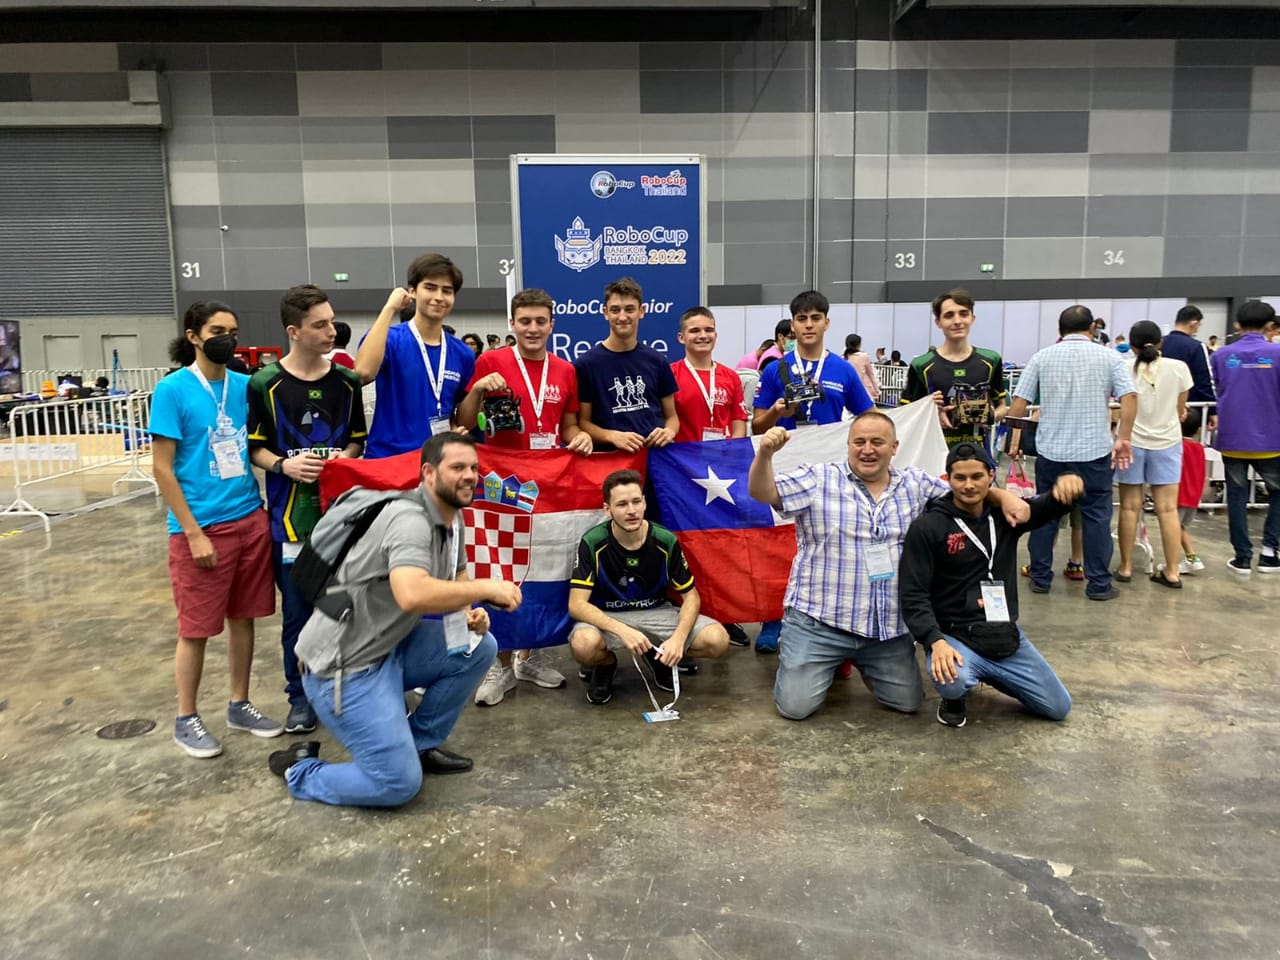
\includegraphics[width=0.5\textwidth]{imagenes_mustabot/competencia2.jpeg}
    \caption{Equipo}
    \label{fig:robot}
\end{figure}

\subsection*{¿Como se elige al equipo mustabot?}
todos los años, se realiza una competencia nacional de clubes, de esta se obtiene al mejor club, el cual es el encargado de representar a Chile
en la competencia internacional.
En los últimos 5 años, Valparaíso (UTFSM) ha sido el encargado de representar a nuestro país.
\begin{figure}[H]
    \centering
    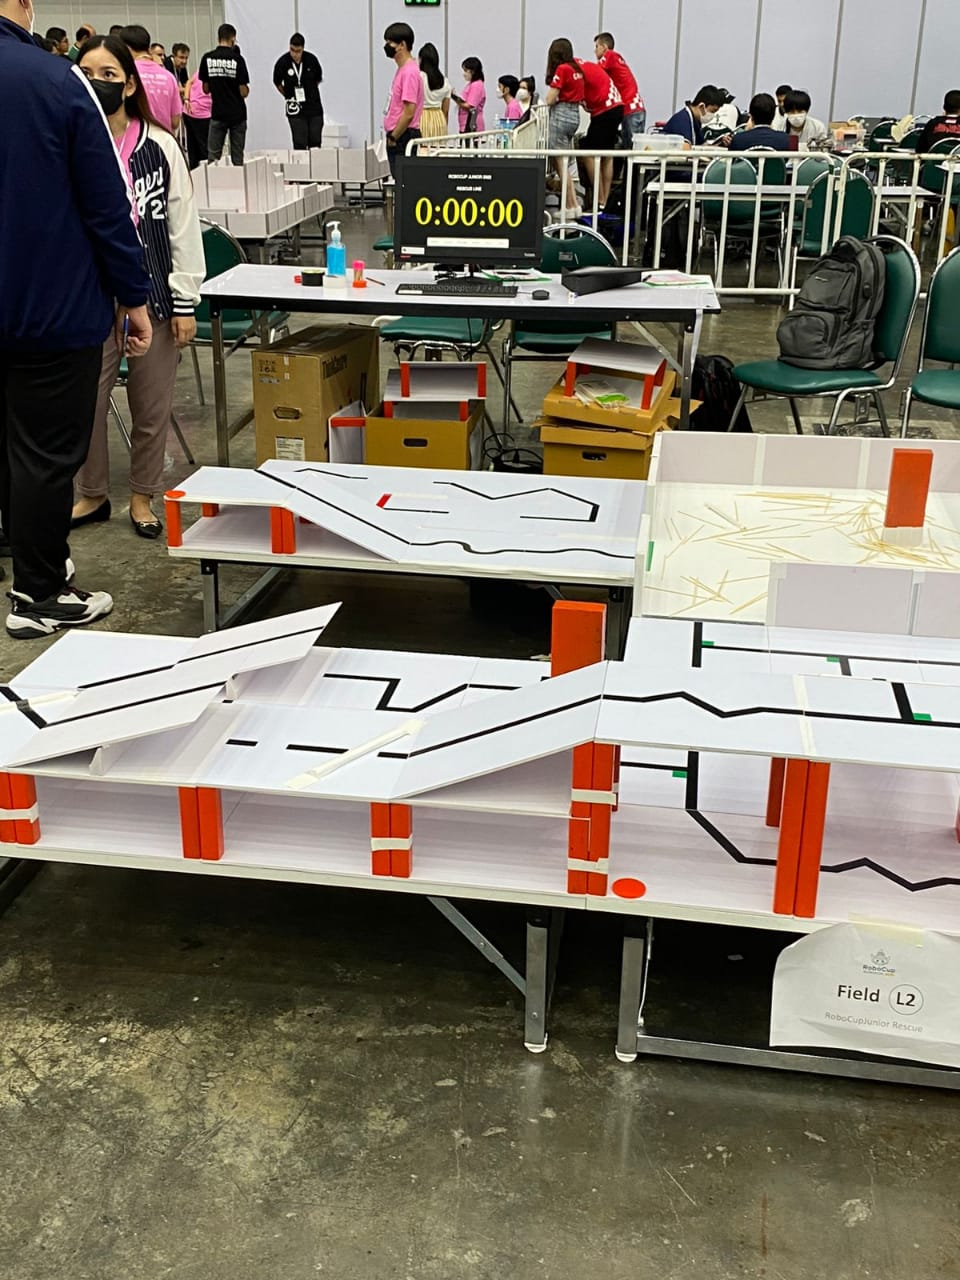
\includegraphics[width=0.5\textwidth]{imagenes_mustabot/competencia.jpeg}
    \caption{Competencia}
    \label{fig:competencia}
\end{figure}

Mustabot Valparaíso ha participado de competencias de robótica desde 2018, representando a Chile en Robocup Rescue Line Junior
en ediciones anteriores han participado otras sedes del país, como Concepción.

\end{document}